
\subsection{Criterio de ambigüedad}

Este último criterio se encarga de detectar y evitar aquellas situaciones en las que la intersección entre un multi-intervalo $A_i$ y un multi-intervalo $B_k$ resulta vacía, considerando un índice $i$ en el rango de $0$ a $|A|$ y un índice $k$ en el rango de $0$ a $|B|$. Y, a pesar de que no hay elementos en común entre estos, no es posible ni descartar $B_k$, es decir aplicar el \textbf{criterio de eliminación}, ni interrumpir la exploración de los elementos restantes en $B$, con respecto a $A_i$ , es decir aplicar el \textbf{criterio de parada}; ya que no cumplen las hipótesis de los criterios.

Para abordar esta problemática con mayor precisión, este criterio se descompone en dos subcriterios más específicos, los cuales se detallan a continuación:

\begin{itemize}
    \item \textbf{Subcriterio de ambigüedad primario:} 

    En algún momento, puede que se llegue a un valor $i$ entre 0 y $|A|$ tal que el elemento mínimo de $A_i$ sea mayor, en alguna componente, que el elemento máximo de $B_k$, para algún $k$ entre 0 y $|B|$. Por ejemplo, que el mínimo de $A_i$ sea $(3,5)$ y el máximo de $B_K$ sea $(3,3)$. Si se da este caso, entonces se pueden concluir lo siguiente:

    \begin{itemize}
    \item No existe intersección entre $A_i$ y $B_k$ porque todos los elementos de $B_K$ son menores que su valor máximo, y todos los elementos de $A_i$ son mayores que su valor mínimo, lo que implica que ningún punto posterior o igual al mínimo de $A_i$ en $A_i$ puede formar parte de $B_k$.
    
    \item Por el orden inherente de los conjuntos, no se puede asegurar de que el multi-intervalo $B_k$ tendra interseccion vacia con los multi-intervalos que le sigan a $A_i$ en $A$.
    \end{itemize}

    \begin{figure}[h]
     \centering
    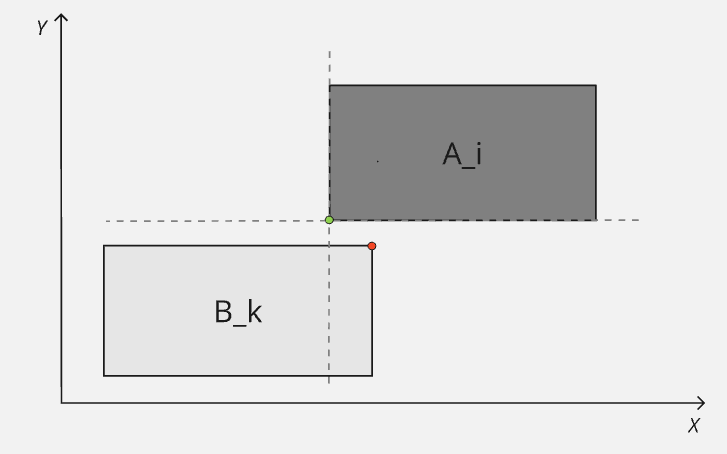
\includegraphics[width=0.6\linewidth]{figures/Optimazaciones/Interseccion/criterio de amb prim 1.png}\par
    \caption{Subcriterio de ambigüedad primario.}
    \label{fig:enter-label}

    \vspace{0.5cm}

    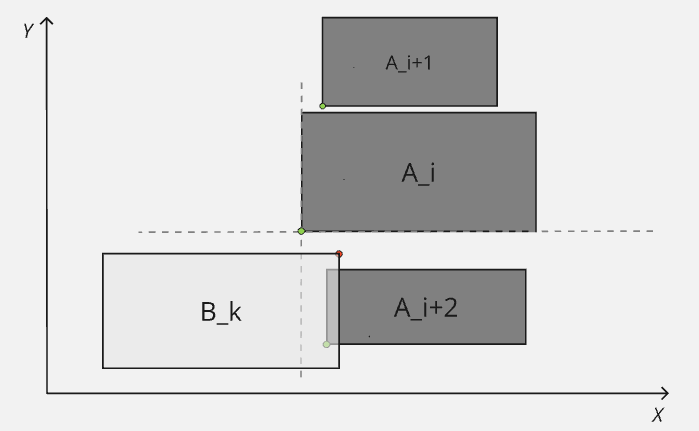
\includegraphics[width=0.6\linewidth]{figures/Optimazaciones/Interseccion/criterio de amb prim 2.png}\par
    \caption{Subcriterio de ambigüedad primario.}
    \label{fig:enter-label}
    
    \end{figure}

    Por lo tanto, no se puede descartar directamente el multi-intervalo $B_k$ como en el criterio de eliminación ya que no se tiene la certeza de que el los siguientes elementos a $A_i$ si tengan una intersección vacía con este como se puede apreciar en la figura mas arriba. Mas concretamente este criterio nos evita realizar el proceso de intersección para $A_i$ y  $B_k$ unicamente.
    

    \item \textbf{Subcriterio de ambigüedad secundario:} 

    En algún momento, puede que se llegue a un valor $k$ entre 0 y $|B|$ tal que el elemento mínimo de $B_k$ sea mayor, en alguna componente, que el elemento mínimo de $A_i$, con $i$ entre 0 y $|A|$. Por ejemplo, que el mínimo de $B_k$ sea $(3,5)$ y el máximo de $A_i$ sea $(3,3)$. Si se da este caso, entonces se pueden concluir lo siguiente:

    \begin{itemize}
    \item No existe intersección entre $A_i$ y $B_k$ porque todos los elementos de $A_i$ son menores que su valor máximo, y todos los elementos de $B_k$ son mayores que su valor mínimo. Esto implica que ningún punto posterior o igual al mínimo de $B_k$ en $B_k$ puede formar parte de $A_i$.
    
    \item Por el orden inherente de los conjuntos, no se puede asegurar de que el multi-intervalo $B_k$ tendrá intersección vacia con los multi-intervalos que le sigan a $A_i$ en $A$.
    \end{itemize}

    \begin{figure}[h]
     \centering
    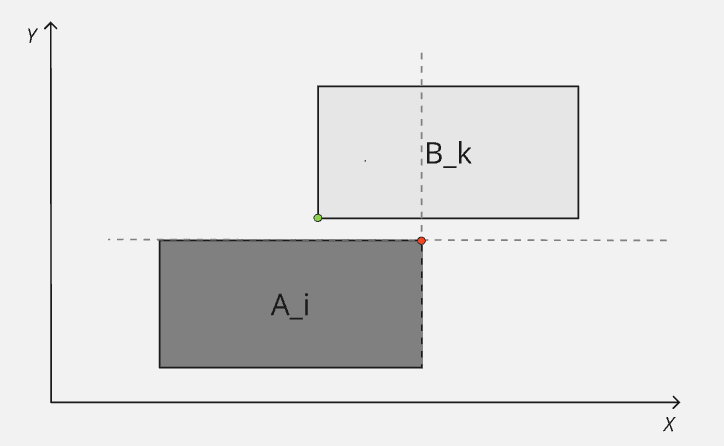
\includegraphics[width=0.6\linewidth]{figures/Optimazaciones/Interseccion/criterio de amb sec 1.png}\par
    \caption{Subcriterio de ambigüedad primario.}
    \label{fig:enter-label}

    \vspace{0.5cm}

    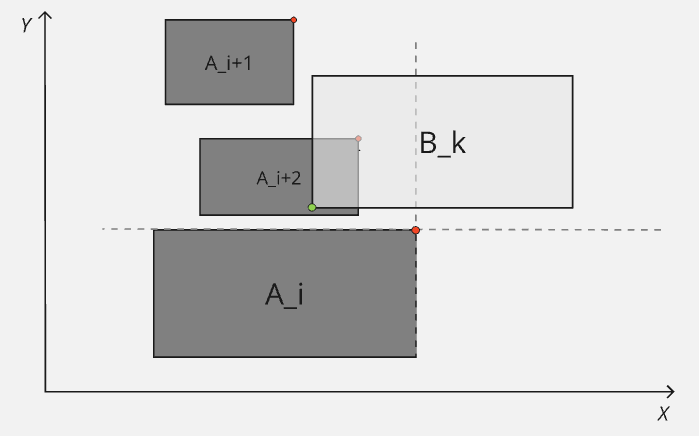
\includegraphics[width=0.6\linewidth]{figures/Optimazaciones/Interseccion/criterio de amb sec 2.png}\par
    \caption{Subcriterio de ambigüedad primario.}
    \label{fig:enter-label}
    
    \end{figure}

    Por lo tanto, no se puede obviar directamente el multi-intervalo $B_k$ y todos los siguientes multi-intervalos a este en $B$ como en el criterio de parada ya que no se tiene la certeza de que el los siguientes elementos a $A_i$ si tengan una intersección vacía con este. Mas concretamente este criterio nos evita realizar el proceso de intersección para $A_i$ y  $B_k$ unicamente.
    
\end{itemize}

Una vez aclarados ambos subcriterios, para aplicar el criterio de ambigüedad los usamos a la par, al ser verdadero uno de ellos, entonces sabemos que no hay intersección entre  $A_i$ y  $B_k$. Cabe destacar que no pueden cumplirse ambos en simultaneo ya que eso significaría que el elemento mínimo de $B_k$ estaría después de su elemento máximo, lo cual no puede pasar.

\chapter{ORDEN PWMAP}

Una vez elegido el dominio como base para definir el orden, restaba establecer un criterio concreto para determinar dicho orden. En particular, se optó por considerar el \textbf{mínimo perimetral} de los dominios de los mapas, pero interpretando los dominios no como conjuntos de múltiples multi-intervalos, sino como conjuntos con un único \textbf{multi-intervalo abstracto} que los contiene a todos. A estos ultimos se lo denominara como \textbf{conjunto abstracto} y por ende el orden de los \textit{piecewise maps} ordenados se basara en esta interpretación de los dominios, en los conjuntos dominio abstractos de los mapas.

Este multi-intervalo abstracto tiene su correspondiente mínimo y máximo, que también son el mínimo y máximo del conjunto abstracto al tener un único elemento. Entonces al mínimo y máximo de un conjunto abstracto se denominaran respectivamente \textbf{mínimo perimetral} y \textbf{máximo perimetral}.  

De esta forma, es posible aplicar nuevamente el criterio de orden definido para conjuntos, pero utilizando como base el mínimo perimetral de los conjuntos dominio abstractos. Esto habilita el uso de optimizaciones análogas a las utilizadas en conjuntos ordenados con \textit{piecewise maps} ordenados.